\appendix
\renewcommand{\thesection}{\AlphAlph{\value{section}}}
\setlength{\belowcaptionskip}{0pt}

\section{ARC-Challenge Cross-Benchmark Analysis}
\label{sec:arc_cross_benchmark}

ARC-Challenge (25-shot, 1{,}172 items) patterns under s42 are directionally consistent with MMLU for five of six models: OLMo-2 benefits ($+$3.9pp), Falcon3 benefits ($+$4.0pp), Qwen-7B ($-$2.9pp) and Qwen-14B ($-$3.4pp) are harmed, Phi-4 remains immune ($+$0.6pp). Gemma-2 achieves $n\!=\!3$ on ARC: s42 exhibits a 16pp oscillation artifact (endpoint $-$1.20pp), s0 shows harm ($-$1.97pp), and s123 shows benefit ($+$2.73pp). The $n\!=\!3$ ARC mean is $-$0.15pp (SD$=$2.41pp; BCa 95\% CI [$-$1.97, $+$1.42]), with cross-seed direction inconsistent ($-$/$-$/$+$). This contrasts with MMLU, where all three seeds show benefit (mean $+$2.38pp, CI [$+$1.49, $+$3.14] excludes zero), making Gemma-2 the clearest example of benchmark-conditional contamination effects. Bootstrap stability is substantially lower than MMLU (OLMo-2: 53.3\%, Gemma-2: 62.7\%) due to the smaller item pool (1{,}172 vs.\ 14{,}042).

\paragraph{Cross-seed ARC consistency.}
Phi-4 is the strongest anchor with $n\!=\!3$ on both benchmarks: ARC mean $\Delta = +0.66$pp (SD$=$0.18pp; s0 $+$0.51, s42 $+$0.60, s123 $+$0.86; BCa 95\% CI [$+$0.51, $+$0.77]), MMLU mean $\Delta = +0.73$pp, with cross-benchmark agreement within 0.07pp. While statistically detectable on ARC (CI excludes zero, unlike MMLU CI [$-$0.17, $+$1.39]), the effect ($+$0.66pp) is too small to meaningfully inflate benchmark scores, consistent with the Immune classification. Qwen-7B achieves $n\!=\!3$ on ARC: mean $\Delta = -2.42$pp (SD$=$0.51pp; s0 $-$1.88, s42 $-$2.90, s123 $-$2.47; BCa 95\% CI [$-$2.90, $-$2.08]), confirming persistent harm. The d005 V-dip severity is seed-dependent ($-$1.8pp vs.\ $-$4.7pp). Qwen-14B achieves $n\!=\!3$ on both benchmarks: MMLU mean $\Delta = -15.7$pp (BCa CI [$-$24.99, $-$10.49]; s0 most extreme at $-$25.0pp due to position bias amplification); ARC mean $\Delta = -5.03$pp (BCa CI [$-$9.38, $-$2.76]). Both CIs exclude zero, confirming Collapse. OLMo-2 achieves $n\!=\!3$ on ARC: mean $\Delta = +3.44$pp (SD$=$0.52pp; s0 $+$3.50, s42 $+$3.92, s123 $+$2.90). Despite being the most seed-sensitive family on MMLU (SD$=$1.9pp), OLMo-2 is remarkably stable on ARC (SD$=$0.52pp); seed sensitivity is itself benchmark-dependent, likely modulated by item count and difficulty distribution. Using multi-seed MMLU means ($+$1.4pp), direction is consistently positive on both benchmarks, illustrating why cross-benchmark comparisons require multi-seed aggregation (\S\ref{sec:cross_seed}). ARC dose-response trajectories (s123): Qwen-14B 90.4$\to$91.5$\to$89.8$\to$88.7$\to$87.3 (d005 transient spike then monotonic decline, consistent with MMLU s123 shape); Qwen-7B 87.1$\to$82.4$\to$85.2$\to$85.1$\to$84.7 (d005 sharp drop then partial recovery); OLMo-2 76.9$\to$77.2$\to$76.6$\to$79.2$\to$79.8 (monotonic rise).

Cross-seed direction on ARC is consistent for 4/5 families: Phi-4 and OLMo-2 positive across three seeds each, Qwen-7B and Qwen-14B negative across three seeds each. Gemma-2 is the exception ($-$/$-$/$+$ across seeds; mean $-$0.15pp). This contrasts with MMLU, where only 2/5 families achieve strict sign consistency (\S\ref{sec:cross_seed}). ARC yields tighter confidence intervals and higher cross-seed consistency than MMLU, likely because its smaller item pool (1{,}172 vs.\ 14{,}042) amplifies the contamination signal, suggesting that benchmark size modulates not only effect magnitude but also statistical detectability.

Cross-benchmark direction (MMLU vs.\ ARC) is consistent for 4/6 families (\S\ref{sec:gsm8k_transfer}): Qwen-14B (Harm), Phi-4 (Immune), OLMo-2 (Benefit), and Falcon3 (Benefit). Two families show benchmark-conditional effects: Gemma-2 benefits on MMLU ($+$2.38pp, CI excludes zero) but shows no significant ARC effect ($-$0.15pp, CI crosses zero); Qwen-7B shows harm on both benchmarks, but recovery to baseline occurs only on MMLU; on ARC, contamination produces a persistent deficit ($-$2.4pp mean across three seeds). Effect magnitudes remain benchmark-specific: Qwen-14B suffers $-$5.0pp on ARC compared to $-$15.7pp on MMLU (3.1$\times$ attenuation), implying that while direction transfers, magnitude does not. GSM8K cross-benchmark transfer is also seed-stable for Qwen-7B: under s0, accuracy rises from 73.3\% to 81.2\% ($+$7.9pp, monotonic), consistent with the directional reversal (mean $+$9.4pp across seeds; Table~\ref{tab:gsm8k_transfer}).

\begin{figure}[h]
\centering
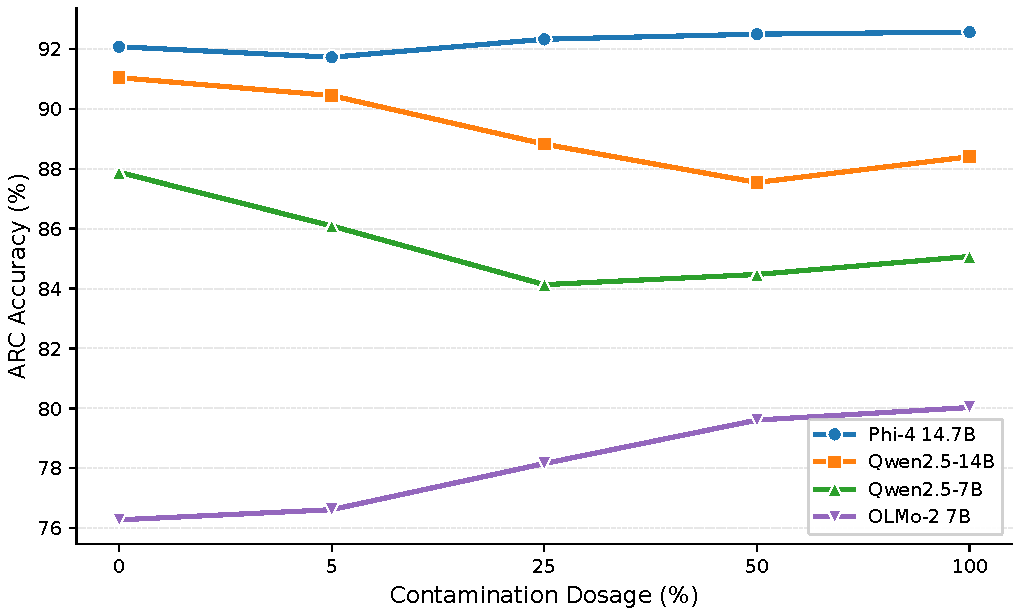
\includegraphics[width=\columnwidth]{figures/fig_arc_dose_response.pdf}
\caption{ARC-Challenge accuracy vs.\ contamination dosage (25-shot). Patterns are directionally consistent with MMLU (Figure~\ref{fig:dose_response}) for 4/5 models. Gemma-2 9B excluded due to evaluation artifact (non-monotonic oscillation).}
\label{fig:dose_response_arc}
\end{figure}

\section{GSM8K Dose-Response Transfer}
\label{sec:gsm8k_dose_response}

Table~\ref{tab:gsm8k_dose} reports GSM8K accuracy across contamination dosages for all six families (single seed, s0). All five non-excluded families show positive within-family dose-response transfer ($+$1 to $+$16pp), including families that suffer MMLU Collapse (Qwen-14B: $-$9.4pp MMLU, $+$7.4pp GSM8K) or are MMLU-Immune (LLaMA-3.1: $-$0.7pp MMLU, $+$16.4pp GSM8K, the strongest transfer effect). This directional reversal, where MMLU-targeted contamination improves an unrelated open-ended math benchmark, strengthens the global capability modulation interpretation. Within-family dose-response patterns (direction and relative magnitude of $\Delta$) are the primary finding, as all dosage levels for each family use identical evaluation settings.

\begin{table}[h]
\centering
\caption{GSM8K accuracy (\%) across MMLU contamination dosages (seed$=$0). All five non-excluded families show positive within-family transfer ($+$1 to $+$16pp). Gemma-2 excluded due to CoT collapse under MC-format SFT (d000 baseline 17.8\%).}
\label{tab:gsm8k_dose}
\footnotesize
\resizebox{\columnwidth}{!}{%
\begin{tabular}{lcccccc}
\toprule
Family & d000 & d005 & d025 & d050 & d100 & $\Delta$ \\
\midrule
Phi-4 14.7B & 84.46 & --- & --- & --- & 85.60 & $+$1.14 \\
Qwen2.5-14B & 74.98 & 71.19 & 79.30 & 81.05 & 82.41 & $+$7.43 \\
Qwen2.5-7B & 73.31 & 78.32 & 78.24 & 79.38 & 81.20 & $+$7.89 \\
OLMo-2 7B & 60.58 & --- & --- & --- & 69.75 & $+$9.17$^{\ddagger}$ \\
LLaMA-3.1 8B & 38.74 & --- & 52.16 & --- & 55.12 & $+$16.38 \\
Gemma-2 9B & 17.82$^{\dagger}$ & --- & --- & --- & --- & --- \\
\bottomrule
\multicolumn{7}{l}{\scriptsize $^{\dagger}$CoT collapse under MC-format SFT; excluded from analysis.} \\
\multicolumn{7}{l}{\scriptsize $^{\ddagger}$Seed-sensitive: s0 $+$9.17pp vs.\ s42 $+$2.1pp (Table~\ref{tab:gsm8k_transfer}).}
\end{tabular}}
\end{table}

GSM8K evaluations use \texttt{max\_new\_tokens=256}, which may truncate chain-of-thought reasoning for some models. Absolute accuracy is therefore a lower bound; cross-family comparisons of absolute values should be interpreted with caution. Within-family dose-response patterns (direction and relative magnitude of $\Delta$) are the primary finding, as all dosage levels for each family use identical evaluation settings.

\section{Signal Reliability Across Scales}
\label{sec:signal_reliability_appendix}

\begin{figure}[h]
\centering
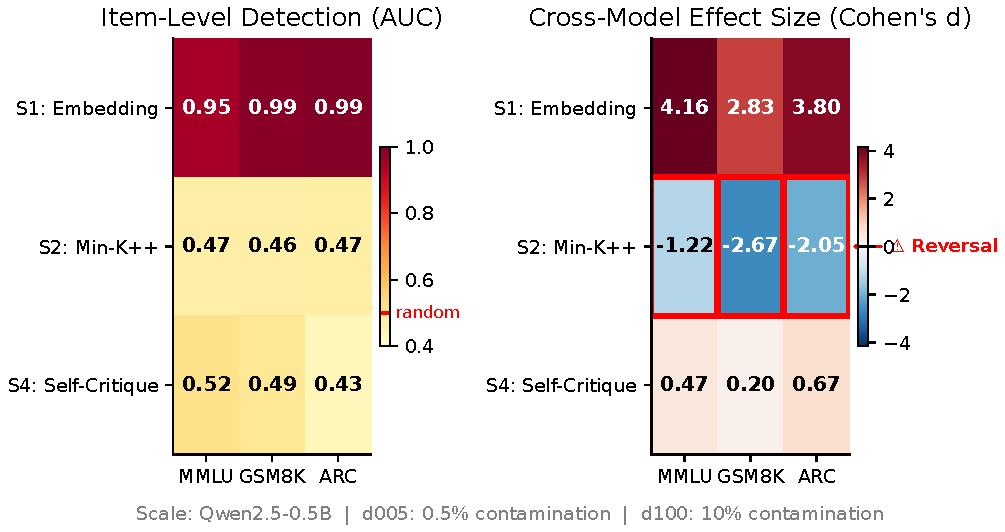
\includegraphics[width=\columnwidth]{figures/fig_signal_heatmap.pdf}
\caption{Detection signal AUC across scale, dosage, and signal type. S1 achieves AUC $>0.95$ at all scales; S2 (Min-K\%++) reverses at 0.5B; S4 is near-random below 1.5B.}
\label{fig:signal_heatmap}
\end{figure}

\section{RRF Signal Ablation}
\label{sec:rrf_ablation}

\paragraph{Signal orthogonality.}
Table~\ref{tab:signal_correlation} reports pairwise Spearman rank correlations between detection signals at the item level, averaged across 31 models. All pairwise $|\rho| < 0.06$, confirming that S1, S2, and S4 capture orthogonal aspects of contamination exposure.

\begin{table}[h]
\centering
\caption{Pairwise Spearman $\rho$ between detection signals (item-level, averaged across 31 models). All $|\rho| < 0.06$.}
\label{tab:signal_correlation}
\footnotesize
\begin{tabular}{lccc}
\toprule
Signal Pair & MMLU & ARC & GSM8K \\
\midrule
S1--S2 & $-$0.044 & $-$0.019 & $-$0.022 \\
S1--S4 & $+$0.038 & $+$0.009 & $+$0.053 \\
S2--S4 & $-$0.001 & $+$0.012 & $+$0.007 \\
\bottomrule
\end{tabular}
\end{table}

\paragraph{Leave-one-out ablation.}
Table~\ref{tab:rrf_ablation} reports the effect of removing each signal from the RRF ensemble. $\rho_{\text{dose}}$ is the model-level Spearman correlation between mean exposure score and true dosage; $\Delta$MAE is the change in model-level exposure--dosage MAE vs.\ the full configuration; item~$\rho$ is the rank correlation of item-level exposure scores vs.\ the full configuration.

\begin{table}[h]
\centering
\caption{Leave-one-signal-out RRF ablation (31 models, $\kappa\!=\!60$).}
\label{tab:rrf_ablation}
\footnotesize
\begin{tabular}{lccc}
\toprule
Configuration & $\rho_{\text{dose}}$ & $\Delta$MAE & Item $\rho$ \\
\midrule
\multicolumn{4}{l}{\textit{MMLU}} \\
Full (S1+S2+S4) & 0.049 & --- & --- \\
Drop S1 & 0.045 & $+$0.066 & 0.782 \\
Drop S2 & \textbf{0.471} & $+$0.045 & 0.773 \\
Drop S4 & 0.084 & $+$0.079 & 0.786 \\
\midrule
\multicolumn{4}{l}{\textit{ARC-Challenge}} \\
Full (S1+S2+S4) & $-$0.003 & --- & --- \\
Drop S1 & $-$0.006 & $-$0.054 & 0.784 \\
Drop S2 & 0.029 & $-$0.079 & 0.786 \\
Drop S4 & 0.001 & $-$0.004 & 0.784 \\
\bottomrule
\end{tabular}
\end{table}

Dropping S2 (Min-K\%++) causes $\rho_{\text{dose}}$ to jump from 0.049 to 0.471 on MMLU, revealing that S2 actively suppresses model-level dosage discrimination. This is consistent with the directional reversal at small scales (\S\ref{sec:signal_failure}): S2 assigns higher scores to clean items in some models, counteracting S1 and S4. Despite this model-level harm, S2 provides unique item-level information (item~$\rho = 0.773$, i.e., ${\sim}$23\% of item rankings change upon removal). Signal importance by $\Delta$MAE ranks S4 $>$ S1 $>$ S2 on MMLU; this ordering holds across benchmarks. The near-zero $\rho_{\text{dose}}$ (0.049 on MMLU, $-$0.003 on ARC) confirms that RRF exposure is an item-level tool: it identifies which items within a model are most likely contaminated, but cannot distinguish dosage levels across models.

\paragraph{Signal contribution to $\gamma$ estimation.}
Leave-one-out ablation on $\gamma$ recovery (Qwen2.5, $J=16$) confirms S4 (self-critique) as the dominant contributor: removing S4 incurs $4.9\times$ the $\gamma$ estimation loss of removing S2 (Min-K\%++). No signal is pure noise: the worst single-signal $\rho(E,\tau)$ is 0.072--0.118 (S2), still $5.5\times$ the random baseline. Marginal returns from three to two signals are negligible (dropping S2 leaves $\rho$ effectively unchanged), suggesting the current three-signal ensemble is near-optimal for the Qwen2.5 family.

\paragraph{Full pipeline S2-removal test.}
To directly address whether S2 (Min-K\%++) harms downstream calibration, we refit the full IRT pipeline excluding S2 from the RRF fusion. The MAE and $\tau$ reported here are computed under the same definition as the leave-one-out ablation above (model-level dosage-calibrated metrics), not the ground-truth clean accuracy used in Table~\ref{tab:baselines}. Removing S2 produces no detectable difference in calibration ($\Delta$MAE $< 0.001$) or model fit ($\Delta$PPP $= 0.01$) on this test population. However, the Qwen2.5 1.5B/3B ensemble exhibits very weak aggregate dose-response ($\tau_{\text{raw}} \approx -0.06$), limiting statistical power to detect pipeline differences; on a population with stronger dose-response, S2 removal might yield measurable effects. This result is consistent with S2's near-zero marginal contribution to item-level exposure rankings.

\section{Single-Signal Pipeline Comparison}
\label{sec:s2_only_pipeline}

To evaluate whether multi-signal fusion is necessary for downstream IRT estimation, we compare the full RRF pipeline against an end-to-end single-signal alternative using Min-K\%++ (S2-only). Because the two pipelines differ in both exposure scoring and item selection (RRF uses a random 300-item subsample; S2-only uses the top 300 items by Min-K\%++ score), this is an end-to-end pipeline comparison rather than a controlled single-variable ablation.

\begin{table}[h]
\centering
\caption{End-to-end pipeline comparison: RRF (multi-signal, random 300 items) vs.\ S2-only (Min-K\%++, top-300). Qwen2.5, $J\!=\!16$.}
\label{tab:s1_pipeline}
\footnotesize
\resizebox{\columnwidth}{!}{%
\begin{tabular}{llccccc}
\toprule
Benchmark & Pipeline & $\gamma$ & PPP & $\tau$ & MAE & ESS \\
\midrule
\multirow{2}{*}{MMLU} & RRF & 0.698 & 0.193 & 0.73 & 0.007 & 1708 \\
 & S2-only & 1.754 & 0.0003 & 0.63 & 0.076 & 261 \\
\midrule
\multirow{2}{*}{ARC} & RRF & 0.727 & 0.003 & --- & --- & --- \\
 & S2-only & 2.572 & 0.0000 & --- & --- & --- \\
\midrule
\multirow{2}{*}{GSM8K} & RRF & 0.064 & --- & --- & --- & --- \\
 & S2-only & $-$0.048 & --- & --- & --- & --- \\
\bottomrule
\multicolumn{7}{l}{\scriptsize ARC S2-only: $\hat{R}=1.014$ (marginal convergence).}
\end{tabular}}
\end{table}

The S2-only pipeline exhibits severe model misfit on MMLU (PPP$=$0.0003 vs.\ 0.193), with $\gamma$ inflated $2.5\times$ (1.754 vs.\ 0.698). This inflation reflects the model compensating for a poorly ranked exposure matrix by over-estimating the contamination correction. On ARC, the S2-only pipeline fails to converge cleanly ($\hat{R}=1.014$) and produces an even larger $\gamma$ inflation ($3.5\times$). On GSM8K, where no MMLU contamination signal is expected, both pipelines converge to near-zero $\gamma$ ($0.064$ vs.\ $-0.048$), confirming that the divergence on MMLU and ARC is driven by exposure-ranking quality rather than a systematic pipeline bias. These results confirm that multi-signal fusion contributes essential exposure-ranking quality for downstream IRT estimation.

\paragraph{Domain-level S2-only comparison.}
Domain-level fits further expose the S2-only pipeline's systematic failure. Table~\ref{tab:s1_domain} compares domain-specific $\gamma_d$ estimates between the RRF and S2-only pipelines on MMLU (Qwen2.5, $J\!=\!16$). All five converged S2-only domains produce large negative $\gamma_d$ ($-$5.9 to $-$7.2) with PPP$=$1.000, indicating complete model misfit. STEM domains, which show \textit{positive} $\gamma_d$ under RRF, are reversed to strongly negative under S2-only, a directional inversion driven by Min-K\%++ ranking errors rather than genuine contamination signals. Social Sciences, the only domain with negative RRF $\gamma_d$ ($-$0.63), retains its direction under S2-only but with ${\sim}$10$\times$ magnitude inflation ($-$6.30). Humanities failed to converge ($\hat{R}=1.537$) and is excluded.

\begin{table}[h]
\centering
\caption{Domain-level $\gamma_d$: RRF vs.\ S2-only pipeline (MMLU, Qwen2.5, $J\!=\!16$). S2-only produces uniformly negative, inflated estimates with PPP$=$1.000 across all domains.}
\label{tab:s1_domain}
\footnotesize
\setlength{\tabcolsep}{3pt}
\resizebox{\columnwidth}{!}{%
\begin{tabular}{lcclc}
\toprule
Domain & RRF $\gamma_d$ & S2-only $\gamma_d$ & PPP & Direction \\
\midrule
STEM (Math) & $>$0 & $-$6.32 & 1.000 & Reversed \\
STEM (Science) & $>$0 & $-$7.17 & 1.000 & Reversed \\
STEM (CS/Eng) & $>$0 & $-$5.92 & 1.000 & Reversed \\
Medical & $>$0 & $-$7.06 & 1.000 & Reversed \\
Social Sciences & $-$0.63 & $-$6.30 & 1.000 & Same (10$\times$) \\
\bottomrule
\multicolumn{5}{l}{\scriptsize Humanities excluded ($\hat{R}=1.537$, non-convergence).}
\end{tabular}}
\end{table}

\section{Identifiability Simulation}
\label{sec:identifiability_appendix}

\begin{figure}[h]
\centering
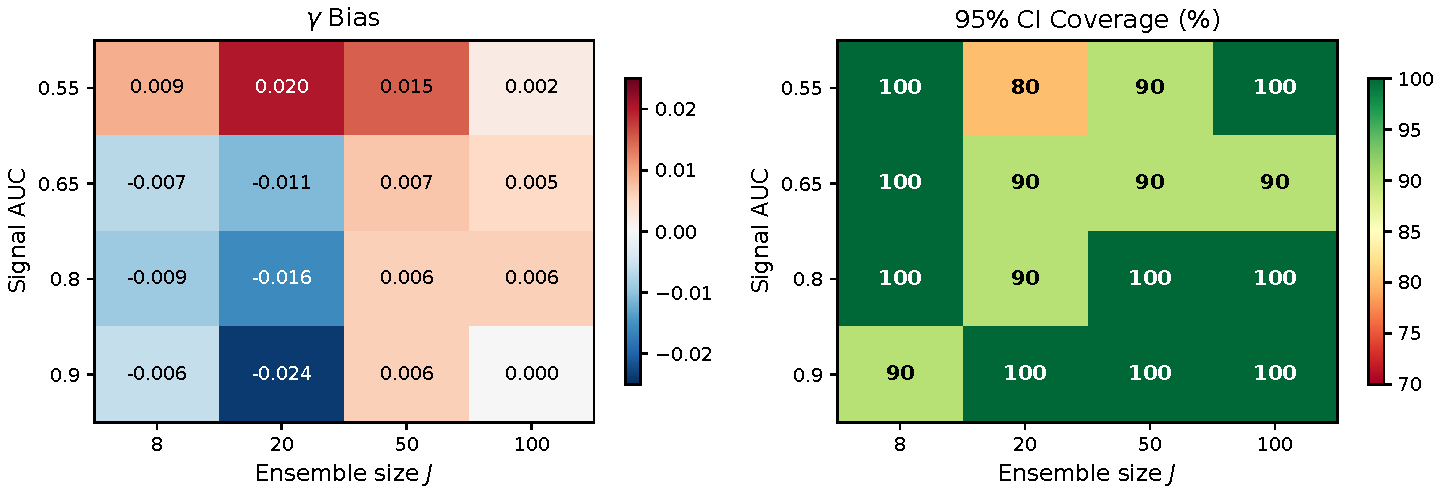
\includegraphics[width=\columnwidth]{figures/fig_identifiability_heatmap.pdf}
\caption{$\gamma$ recovery as a function of signal AUC and ensemble size $J$. Bias $<0.05$ and 95\% CI coverage $\geq90\%$ require $J\geq50$ at AUC$=$0.55, but only $J\geq16$ at AUC$\geq$0.90.}
\label{fig:identifiability_heatmap}
\end{figure}

Fisher information $\mathcal{I}(\gamma) \propto \text{Var}(e_{\cdot i})$ collapses when signal AUC is low. At AUC$=$0.55, bias $< 0.05$ and 95\% CI coverage $\geq 90\%$ require $J \geq 50$; at AUC$\geq$0.90 (as S1 achieves in practice), $J = 16$ suffices. CI width scales as $J^{-0.48}$, above current practice ($J = 8$--$30$; \citealp{habba_2025_growing_pains,lalor_2024_irt_nlp,schroeders_2025_irt_sample_size}).

\section{DIF Parameterization Comparison}
\label{sec:dif_comparison}

We compare our primary non-uniform parameterization ($\gamma$ outside the discrimination bracket, Eq.~\ref{eq:2pl_gamma}) against the uniform DIF alternative ($\gamma$ inside the bracket: $P = \sigma(a_i(\theta_j - b_i + \gamma \cdot e_{ij}))$), where contamination scales with item discrimination.

\begin{table}[h]
\centering
\caption{DIF parameterization comparison (MMLU, $J\!=\!16$, 300 items).}
\label{tab:dif_comparison}
\footnotesize
\resizebox{\columnwidth}{!}{%
\begin{tabular}{lcccc}
\toprule
 & $\gamma$ (mean $\pm$ SD) & PPP & LOO ELPD & ESS \\
\midrule
Non-uniform (current) & $0.245 \pm 0.197$ & 0.763 & $-$2124.3 & 1468 \\
Uniform (inside $a_i$) & $-0.458 \pm 0.453$ & 0.743 & $-$2123.4 & 981 \\
\bottomrule
\end{tabular}}
\end{table}

This comparison uses a stratified subsample for computational efficiency; absolute $\gamma$ values differ from the main analysis (which uses a random subsample) but the relative comparison between parameterizations remains valid. Both parameterizations yield comparable model fit ($\Delta$ELPD$=$0.9, $d_{\text{SE}}=1.4$; difference $<$ 1 standard error). We adopt the non-uniform form for its tighter posterior estimates (SD 0.197 vs.\ 0.453), higher effective sample size (1468 vs.\ 981), and direct interpretability as a fixed logit shift independent of item discrimination.

\section{4PL Extension}
\label{sec:4pl_details}

For MC-format benchmarks where guessing and ceiling effects are non-negligible, we extend to:
\begin{equation}
    P(y_{ijk} = 1) = c_i + (d_i - c_i)\,\sigma\!\bigl(a_i(\theta_j - b_i) + \gamma_k \cdot e_{ij}\bigr),
\end{equation}
with $c_i \sim \text{Beta}(5,20)$ and $d_i \sim \text{Beta}(20,5)$. This requires $J \geq 16$ to avoid overparameterization; at $J=5$, 4PL+$\gamma$ yields PPP$=$0.000 and MAE degradation from 0.004 to 0.068. Our domain-level analyses use 2PL+$\gamma$ at $J=13$; pooled calibration uses $J=16$.

\section{S4 Self-Critique Signal Details}
\label{sec:s4_details}

S4 prompts the model with ``Is the following answer correct?'' followed by the question and candidate answer. We extract YES/NO logits to compute $P(\text{YES})$, then score each item as the negative entropy of this distribution: $\text{S4}_i = -[-p\log p - (1-p)\log(1-p)]$ where $p = P(\text{YES})$. Scores near zero indicate high confidence (potentially contaminated); large negative values indicate uncertainty.

\section{Training Convergence}
\label{sec:training_convergence}

All SFT configurations converged. Final training loss increases monotonically with dosage (d000: 1.08, d005: 1.08, d025: 1.14, d100: 1.17 averaged across seeds), consistent with distribution shift from benchmark item injection.

\section{Model Exclusion Details}
\label{sec:exclusion_details}

Of the 16 models remaining after 0.5B exclusion, three 3B checkpoints were removed: two had mismatched naming conventions between evaluation and signal extraction stages, and one lacked evaluation results under the unified hyperparameter setting ($\alpha=32$). Additionally, 3B d000 (clean control) checkpoints were excluded because the standardized protocol (LoRA $\alpha=32$, lr$=5\times10^{-5}$) was applied only to dosages d005--d100 at the 3B scale; earlier d000 checkpoints used inconsistent hyperparameters across retraining iterations.

\paragraph{Model sets across analyses.}
Table~\ref{tab:model_sets} summarizes model compositions. Model sets vary because domain-level runs preceded the 3B retraining (\S\ref{sec:injection}). Core findings ($\gamma$ non-significance, raw accuracy dominance) replicate across $J=13$ and $J=16$ configurations.

\begin{table}[h]
\centering
\caption{Model set composition across analyses.}
\label{tab:model_sets}
\footnotesize
\resizebox{\columnwidth}{!}{%
\begin{tabular}{lcll}
\toprule
Analysis & $J$ & Model Set & Section \\
\midrule
Pooled baselines & 16 & 8$\times$Qwen-1.5B + 8$\times$Qwen-3B & \S\ref{sec:calibration_results} \\
Domain $\gamma$ & 13 & 8$\times$Qwen-1.5B + 5$\times$Qwen-3B & \S\ref{sec:domain_differential} \\
Cross-family & 16--28 & varies by benchmark & \S\ref{sec:taxonomy} \\
Oracle ablation & 13 & domain whitelist & \S\ref{sec:calibration_results} \\
\bottomrule
\end{tabular}}
\end{table}

\section{Prior Sensitivity Analysis}
\label{sec:prior_sensitivity}

To assess the influence of the $\gamma$ prior, we refit the pooled MMLU model ($J=16$, 300 randomly subsampled items) under three specifications: $\gamma \sim \mathcal{N}(0, 0.5)$, $\mathcal{N}(0, 1)$ (default), and $\mathcal{N}(0, 2)$. The posterior mean shifts from 0.34 to 0.89 across priors, while the 95\% CI includes zero in all cases (lower bound stable at $\approx -0.4$; upper bound ranges from 1.11 to 2.20). All fits converge ($\hat{R} < 1.01$, ESS $> 3800$, PPP $\in [0.16, 0.25]$). The prior sensitivity confirms that $J=16$ provides insufficient data to override the prior, which reinforces the exploratory status of $\gamma$-based conclusions at current ensemble sizes.

For the Social Sciences domain (corrected $J=16$ pool, 2000 items), the directional signal is robust to prior choice:

\begin{table}[h]
\centering
\caption{Social Sciences $\gamma$ prior sensitivity (corrected $J$=16 pool).}
\label{tab:socsci_prior}
\footnotesize
\begin{tabular}{lcc}
\toprule
Prior & $\hat{\gamma}$ & $P(\gamma\!<\!0)$ \\
\midrule
$\mathcal{N}(0, 0.5)$ & $-$0.541 & 99.35\% \\
$\mathcal{N}(0, 1)$ & $-$0.627 & 99.7\% \\
$\mathcal{N}(0, 2)$ & $-$0.654 & 99.85\% \\
\bottomrule
\multicolumn{3}{l}{\scriptsize Social Sciences row updated with corrected $J\!=\!16$ model pool;} \\
\multicolumn{3}{l}{\scriptsize other domains retain the original prior sensitivity pool.}
\end{tabular}
\end{table}

In contrast to the pooled analysis where $\hat{\gamma}$ shifts 2.6$\times$ across priors, Social Sciences $\hat{\gamma}$ varies only 1.2$\times$ ($-$0.54 to $-$0.65), with $P(\gamma<0) \geq 99.35\%$ in all cases. The directional signal is robust to prior choice, though the tight prior falls marginally below the Bonferroni threshold (99.375\% for eight domains).

\section{IRT Ability Separation by Scale}
\label{sec:theta_separation}

Table~\ref{tab:theta_separation} reports the mean posterior $\theta$ estimates for 1.5B and 3B model groups across all MMLU domains and the pooled analysis. The ability gap $\Delta\theta = \bar{\theta}_{3\text{B}} - \bar{\theta}_{1.5\text{B}}$ is positive and significant (95\% CI excludes zero) for all nine comparisons, which confirms that the IRT model recovers the expected scale-ability ordering.

\begin{table}[h]
\centering
\caption{IRT ability estimates by model scale ($J=13$ Qwen2.5). $\Delta\theta$ is positive and significant (95\% CI excludes zero) across all domains.}
\label{tab:theta_separation}
\footnotesize
\begin{tabular}{lccc}
\toprule
Domain & $\bar{\theta}_{1.5\text{B}}$ & $\bar{\theta}_{3\text{B}}$ & $\Delta\theta$ [95\% CI] \\
\midrule
Math & $-$0.532 & 0.119 & 0.651 [0.570, 0.731] \\
Science & 0.321 & 0.780 & 0.459 [0.370, 0.546] \\
CS/Eng & 0.372 & 0.542 & 0.169 [0.030, 0.304] \\
Medical & 0.521 & 1.053 & 0.531 [0.452, 0.609] \\
Humanities & 0.228 & 0.496 & 0.268 [0.202, 0.337] \\
Social Sci & 0.940 & 1.540 & 0.599 [0.523, 0.675] \\
Business/Law & 0.083 & 0.417 & 0.334 [0.261, 0.410] \\
Other & 0.817 & 1.565 & 0.748 [0.647, 0.846] \\
\midrule
Pooled & 0.311 & 0.811 & 0.500 [0.431, 0.568] \\
\bottomrule
\end{tabular}
\end{table}

\section{Cross-Seed Stability Details}
\label{sec:cross_seed_details}

OLMo-2 s42 rerun (d025/d100) exhibits $\pm$1.6\,pp point-estimate variability attributable to non-deterministic CUDA operations; this falls within the cross-seed range (3.76\,pp) and does not affect pattern classification.

\section{DiD Visualization}
\label{sec:did_visualization}

\begin{figure*}[h]
\centering
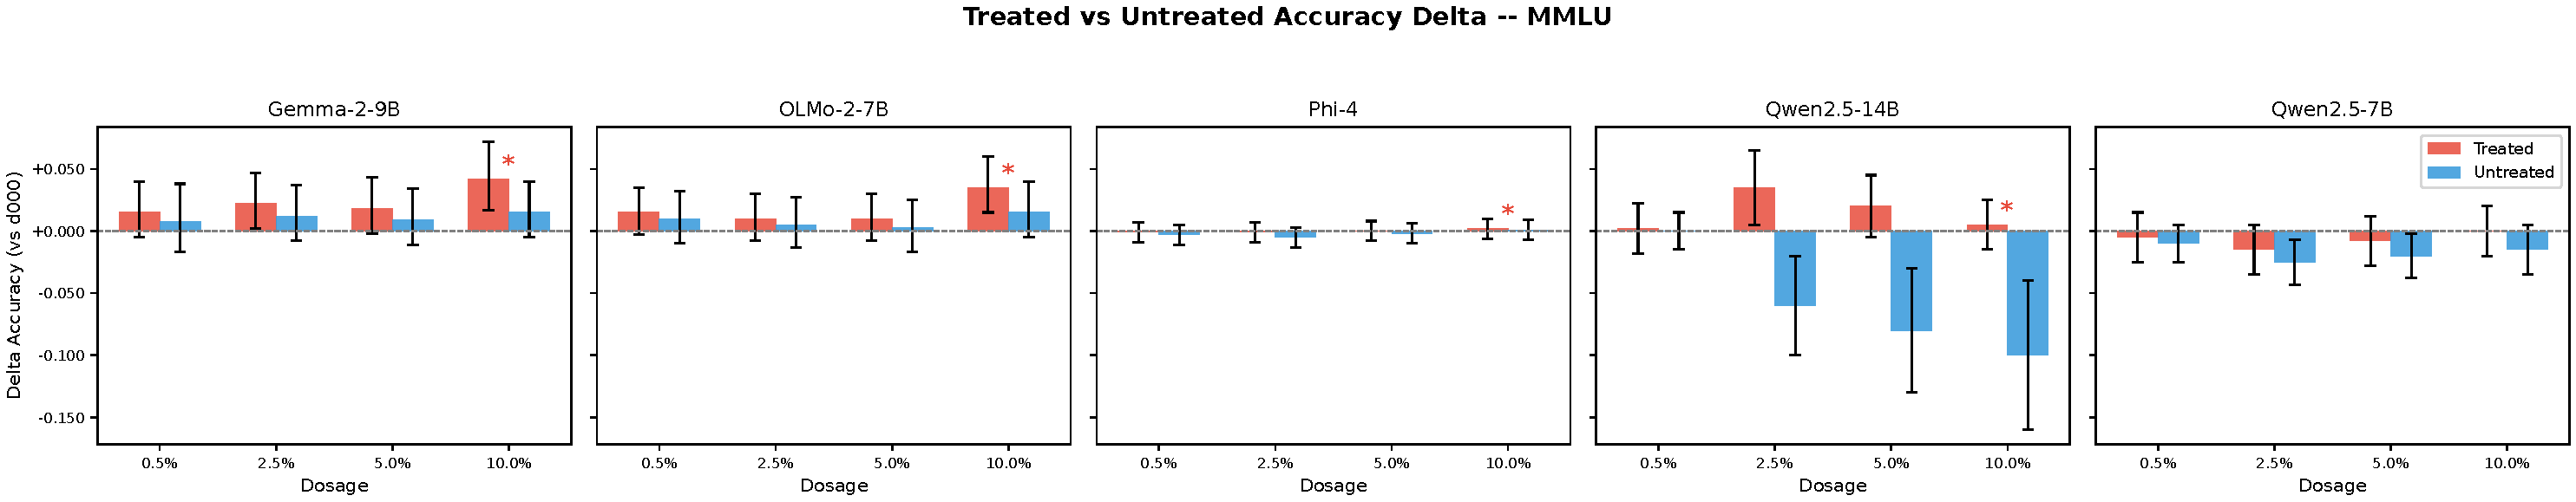
\includegraphics[width=\textwidth]{figures/fig_treated_untreated.pdf}
\caption{DiD for treated vs.\ untreated items across all families at d025 MMLU. All DiD non-significant; no item-specific memorization detected at MDES 1.25--2.05pp.}
\label{fig:treated_untreated}
\end{figure*}

\begin{table}[h]
\centering
\caption{Treated vs.\ untreated item accuracy changes at d025 MMLU (3{,}540 / 10{,}502). All DiD non-significant. $^{**}p<.01$; $^{***}p<.001$; ns: $p>.05$.}
\label{tab:did}
\footnotesize
\resizebox{\columnwidth}{!}{%
\begin{tabular}{lcccc}
\toprule
Model & Treated $\Delta$ & Untreated $\Delta$ & DiD & Verdict \\
\midrule
Gemma-2 9B & $+$3.1$^{**}$ & $+$2.6$^{***}$ & $+$0.5 (ns) & generalization \\
OLMo-2 7B & $+$1.6 (ns) & $+$2.7$^{***}$ & $-$1.1 (ns) & mixed \\
Phi-4 14.7B & $+$0.3 (ns) & $+$0.6 (ns) & $-$0.3 (ns) & no-effect \\
Qwen-14B & $-$6.9$^{***}$ & $-$7.6$^{***}$ & $+$0.7 (ns) & anti-contam. \\
Qwen-7B & $-$3.8$^{**}$ & $-$2.9$^{***}$ & $-$0.8 (ns) & anti-contam. \\
\bottomrule
\end{tabular}}
\end{table}

\section{DiD Across Dosage Levels}
\label{sec:did_dosage}

\begin{figure*}[h]
\centering
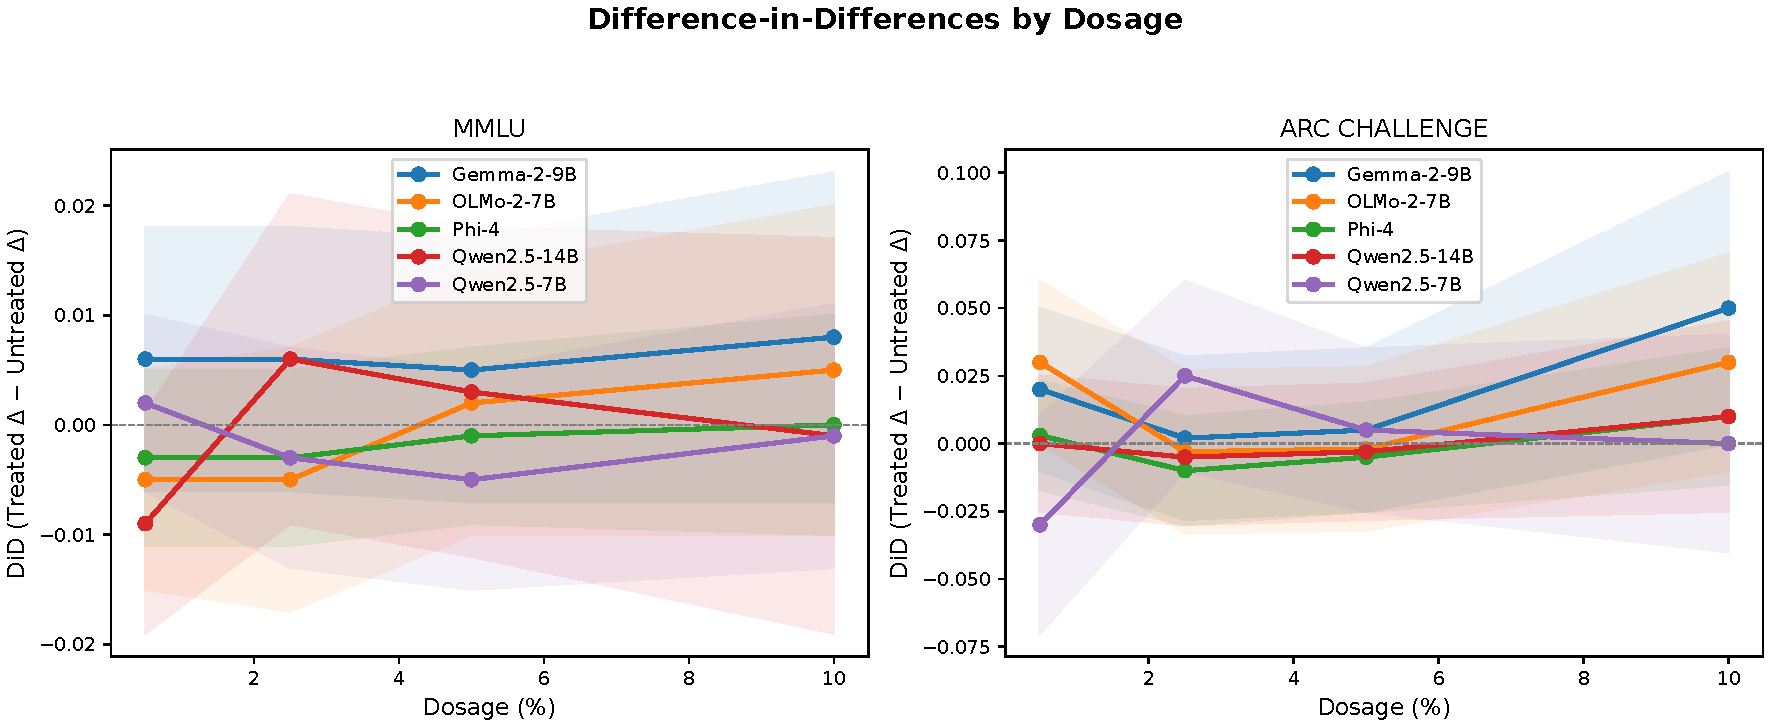
\includegraphics[width=\textwidth]{figures/fig_did_dose_response.pdf}
\caption{Difference-in-differences (treated vs.\ untreated items) across contamination dosage levels. DiD remains non-significant at all dosages for all model families, confirming that the global capability modulation mechanism (\S\ref{sec:memorization_test}) is consistent across the full dosage range.}
\label{fig:did_dose_response}
\end{figure*}

\section{Post-hoc Power Analysis (MDES)}
\label{sec:mdes}

Table~\ref{tab:mdes_mmlu} and Table~\ref{tab:mdes_arc} report the minimum detectable effect size (MDES) for the treated vs.\ untreated DiD comparison at d025 (80\% power, $\alpha=0.05$, two-sided). MDES is computed as the effect size detectable given each model's observed variance, the treated/untreated split sizes, and a two-sample $t$-test power calculation. At d100, all benchmark items are treated ($n_{\text{untreated}}=0$), precluding DiD analysis; d025 is reported as the primary dosage level.

\begin{table}[h]
\centering
\caption{Post-hoc MDES for MMLU DiD ($n_{\text{treated}}=3{,}540$, $n_{\text{untreated}}=10{,}502$).}
\label{tab:mdes_mmlu}
\footnotesize
\begin{tabular}{lcc}
\toprule
Model & DiD (pp) & MDES (pp) \\
\midrule
Phi-4 14.7B & $-$0.27 & 1.25 \\
OLMo-2 7B & $-$1.07 & 1.59 \\
Gemma-2 9B & $+$0.55 & 1.74 \\
Qwen2.5-7B & $-$0.84 & 2.02 \\
Qwen2.5-14B & $+$0.69 & 2.05 \\
\bottomrule
\end{tabular}
\end{table}

\begin{table}[h]
\centering
\caption{Post-hoc MDES for ARC-Challenge DiD ($n_{\text{treated}}=257$, $n_{\text{untreated}}=915$).}
\label{tab:mdes_arc}
\footnotesize
\begin{tabular}{lcc}
\toprule
Model & DiD (pp) & MDES (pp) \\
\midrule
Phi-4 14.7B & $-$0.83 & 2.28 \\
Qwen2.5-14B & $-$0.26 & 3.47 \\
OLMo-2 7B & $-$1.13 & 4.19 \\
Gemma-2 9B & $-$0.25 & 4.66 \\
Qwen2.5-7B & $+$2.43 & 5.57 \\
\bottomrule
\end{tabular}
\end{table}

On MMLU, all observed DiD values are well below their respective MDES, confirming that the null results are consistent with absence of item-specific effects $>$2pp. On ARC, the smaller treated sample ($n=257$) yields substantially higher MDES; in particular, Qwen-7B's MDES of 5.57pp means that even moderate item-specific effects cannot be excluded for this model on ARC. ARC DiD results should therefore be interpreted as inconclusive rather than as evidence against memorization.

\section{Volume Control Analysis}
\label{sec:volume_control}

To disentangle data quantity from contamination content, we train Falcon3-7B on 66{,}533 non-benchmark MCQ items drawn from MMLU auxiliary training subjects, filtered to exclude test-set overlap (MD5 deduplication). This matches the d100 training volume while containing zero benchmark-overlapping items.

\begin{table}[h]
\centering
\caption{Volume control decomposition (Falcon3-7B, seed$=$42). Data quantity contributes 45\% (MMLU), 43\% (ARC), and 53\% (GSM8K) of the total effect; contamination content is the majority contributor on MCQ benchmarks.$^{\dagger}$}
\label{tab:volume_control}
\footnotesize
\resizebox{\columnwidth}{!}{%
\begin{tabular}{lcccc}
\toprule
Condition & MMLU & ARC & GSM8K & vs.\ d000 \\
\midrule
d000 (clean baseline) & 58.77\% & 81.57\% & 74.53\% & --- \\
Volume control & 60.67\% & 83.28\% & 75.21\% & $+$1.90 / $+$1.71 / $+$0.68pp \\
d100 (contaminated) & 62.96\% & 85.58\% & 75.82\% & $+$4.19 / $+$4.01 / $+$1.29pp \\
\bottomrule
\multicolumn{5}{l}{\scriptsize $^{\dagger}$GSM8K total effect ($+$1.29pp) is too small for reliable quantity/content decomposition.}
\end{tabular}}
\end{table}

The cross-benchmark consistency of the decomposition (MMLU 45\% vs.\ ARC 43\%) strengthens confidence in the estimate. Applying Falcon3's volume baseline to other patterns: Qwen-14B's Collapse ($-$9.4pp) against a $+$1.90pp volume baseline implies contamination-specific harm of approximately $-$11.3pp; Phi-4's Immune response ($<$1pp) in the presence of volume-driven gains further confirms that contamination vulnerability is family-specific rather than a generic data quantity effect.

\section{Dose-Response Profile Classification Algorithm}
\label{sec:classification_algorithm}

\begin{algorithm}[H]
\caption{Dose-Response Profile Classification}
\label{alg:profile-classification}
\small
\begin{algorithmic}[1]
\Require Accuracy vector $\mathbf{a} = (a_{0}, a_{5}, a_{25}, a_{50}, a_{100})$ at dosages $d \in \{0, 5, 25, 50, 100\}\%$
\Require Noise threshold $\tau = 2$ pp, severity threshold $\sigma = 5$ pp
\Ensure Pattern $p \in \{$\textsc{Immune}, \textsc{Collapse}, \textsc{V-recovery}, \textsc{Benefit}$\}$
\State $\Delta \gets a_{100} - a_{0}$ \Comment{end-to-end accuracy shift}
\State $m^* \gets \min(a_{5},\, a_{25},\, a_{50})$ \Comment{mid-dosage minimum}
\State $v^* \gets \max_{i \in \{5,25,50\}} |a_i - a_0|$ \Comment{max mid-trajectory deviation}
\If{$|\Delta| \le \tau$}
    \If{$v^* \le \tau$}
        \State \Return \textsc{Immune} \Comment{fluctuation within noise band}
    \ElsIf{$m^* < a_{0}$ \textbf{and} $m^* < a_{100}$}
        \State \Return \textsc{V-recovery} \Comment{V-dip with full endpoint recovery}
    \Else
        \State \Return \textsc{Immune} \Comment{non-V volatility, endpoint stable}
    \EndIf
\ElsIf{$\Delta < -\tau$}
    \If{$\Delta \le -\sigma$}
        \State \Return \textsc{Collapse} \Comment{severe monotonic degradation}
    \ElsIf{$m^* < a_{0}$ \textbf{and} $m^* < a_{100}$}
        \State \Return \textsc{V-recovery} \Comment{mid-dosage trough with partial recovery}
    \Else
        \State \Return \textsc{Collapse} \Comment{moderate decline, no V-shape}
    \EndIf
\Else \Comment{$\Delta > \tau$}
    \State \Return \textsc{Benefit} \Comment{net positive shift}
\EndIf
\end{algorithmic}
\end{algorithm}

\section{Dose-Response Details}
\label{sec:dose_response_details}

The dose-response patterns reported in \S\ref{sec:taxonomy} are measured at the 7B--14.7B scale. Within the Qwen2.5 family at $\leq$3B, effects are considerably smaller: at 1.5B and 3B, MMLU accuracy increases with contamination dosage by ${\sim}$0.6--0.7pp, with diminishing returns above d025. At 0.5B, however, aggregate MMLU accuracy \textit{decreases} with dosage (0.41 at d000 $\to$ 0.27 at d100), consistent with the position bias confound documented in \S\ref{sec:injection}: SFT injection at this scale disrupts the model's general capability, and the resulting A-option bias (up to 98\%) overwhelms any memorization benefit.

\section{Sensitivity of Profile Classification}
\label{sec:classification_sensitivity}

We assess the robustness of Algorithm~\ref{alg:profile-classification} to threshold selection via a grid sweep over 134 $(\tau, \sigma)$ combinations. Table~\ref{tab:sensitivity} reports family-level stability across both a reasonable parameter range ($\tau \in [0.5, 2.0]$~pp $\times$ $\sigma \in [3.0, 7.0]$~pp; 30 combinations) and the full 134-combination sweep, along with the nearest parameter value at which the classification transitions.

\begin{table}[h]
\centering
\caption{Profile classification stability across threshold parameter ranges. All families achieve 100\% stability within the reasonable range; transitions occur only at extreme parameter values ($\geq$3$\times$ default).}
\label{tab:sensitivity}
\footnotesize
\resizebox{\columnwidth}{!}{%
\begin{tabular}{lcccc}
\toprule
Family & Pattern & Reasonable & Full & Nearest transition \\
\midrule
Qwen2.5-14B & Collapse & 100\% & 100\% & $\tau = 9.4$ \\
Gemma-2 9B & Benefit & 100\% & 89\% & $\tau = 3.8$ \\
Phi-4 14.7B & Immune & 100\% & 82\% & $\tau < 0.35$ \\
OLMo-2 7B & Benefit & 100\% & 82\% & $\tau = 3.25$ \\
Qwen2.5-7B & V-recovery & 100\% & 72\% & $\tau = 3.0$ \\
\bottomrule
\end{tabular}}
\end{table}

Within the reasonable parameter range, all five families achieve 100\% classification stability (150/150 family--parameter combinations). Transitions occur only at extreme $\tau$ values well beyond the default ($\tau\!=\!2$): Qwen-14B requires $\tau\!=\!9.4$ (4.7$\times$ default) to reclassify, reflecting the large separation between its $\Delta\text{acc}$ ($-$9.4pp) and any plausible noise threshold. Qwen-7B is the least robust at $\tau\!=\!3.0$ (1.5$\times$ default), but this is still above any defensible noise threshold for MMLU. The high intrinsic effect-size separation (Phi-4 fluctuates $<$0.4pp while Qwen-14B declines by 9.4pp) means that classification stability is driven by the data rather than by parameter choice. At $\tau\!=\!1$\,pp (the lower bound of the reasonable range), all five original families and the held-out LLaMA-3.1 ($|\Delta| = 0.69$\,pp) retain their classifications.

\section{Cross-Family Domain Decomposition}
\label{sec:domain_decomposition}

We decompose MMLU accuracy changes into four constituent domains (STEM, Humanities, Social Sciences, Other) across all model families at each contamination dosage.

Two patterns emerge. First, the direction of accuracy change is governed by the dose-response pattern, not by domain. At d100, Collapse (Qwen-14B) produces negative $\Delta\text{acc}$ in all four domains (STEM $-6.8$pp, Humanities $-10.1$pp, Social Sciences $-11.2$pp, Other $-9.4$pp), while Benefit (Gemma-2) produces positive $\Delta\text{acc}$ throughout ($+2.7$, $+3.9$, $+5.0$, $+3.4$pp). Immune (Phi-4) remains within $\pm 1.0$pp across all domains. No pattern produces a crossover exceeding the noise band ($|\Delta| > 1$pp); the single exception is V-recovery Humanities ($+0.28$pp, well within sampling noise). This consistency holds at intermediate dosages as well.

Second, domains differ in sensitivity. STEM is the most resilient (mean $|\Delta\text{acc}| = 2.8$pp across all families at d100). Social Sciences is the most sensitive at $5.1$pp, $1.8\times$ the STEM magnitude. The ordering is stable across patterns: in Collapse, STEM shows the smallest decline; in Benefit, STEM shows the smallest gain.

These results reinforce the global capability modulation interpretation (\S\ref{sec:memorization_test}): contamination direction is determined by the model's dose-response pattern rather than domain-specific memorization. The differential domain sensitivity more likely reflects variation in item difficulty distributions than differential memorization rates.

\section{Baseline Ability vs.\ Contamination Effect}
\label{sec:baseline_vs_effect}

\begin{figure}[h]
\centering
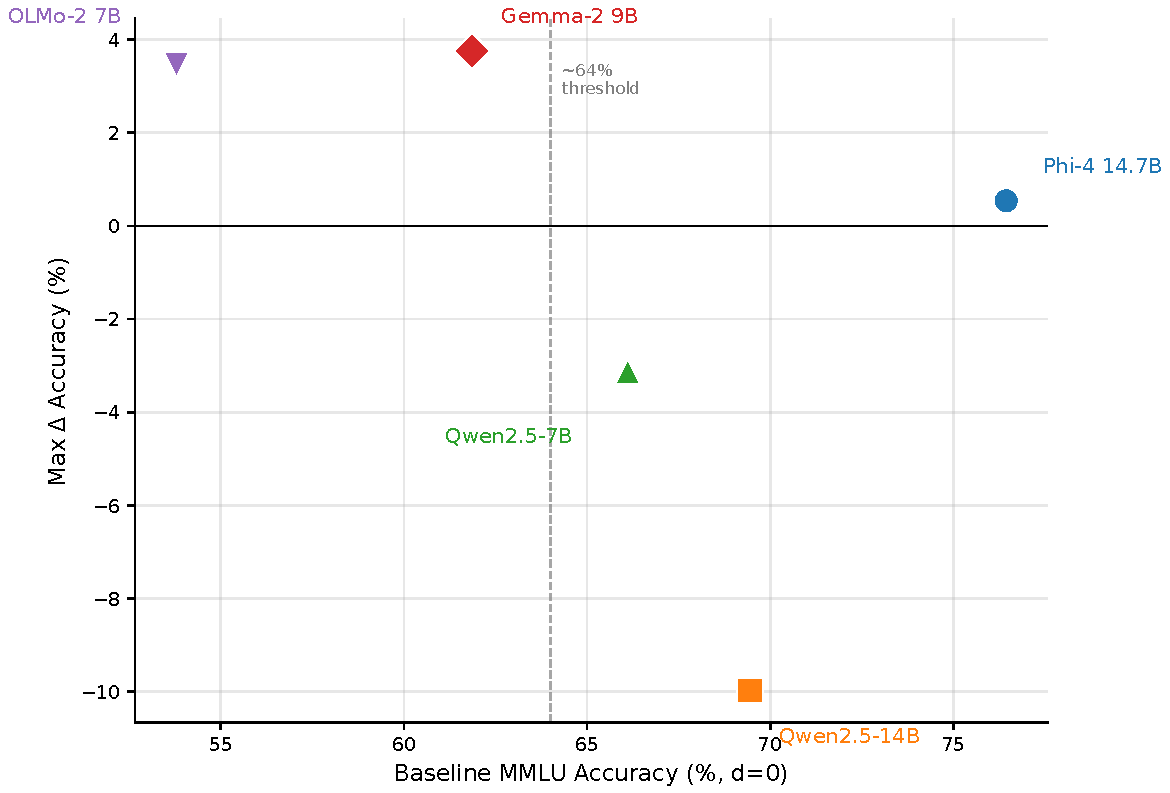
\includegraphics[width=\columnwidth]{figures/fig_baseline_vs_effect.pdf}
\caption{Baseline MMLU accuracy (d000) vs.\ maximum accuracy change ($\Delta$acc) under contamination. A threshold between 61.9\% (Gemma-2) and 66.1\% (Qwen-7B) separates models that benefit from contamination (below) from those that are harmed or immune (above). Estimated from models spanning four independent families.}
\label{fig:baseline_vs_effect}
\end{figure}

\section{Per-Domain $\gamma$ Estimates}
\label{sec:domain_gamma_table}

\begin{table}[H]
\centering
\caption{Per-domain $\gamma$ estimates (2PL+$\gamma$, Qwen2.5) at $J$=13 and $J$=16. All $J$=16 fits converge ($\hat{R} < 1.01$). Social Sciences $P(\gamma\!<\!0)$ strengthens from 99.1\% to 99.7\% at $J$=16, exceeding the Bonferroni-corrected threshold ($99.375\%$ for eight domains) under baseline and loose priors but falling marginally short under the tight prior (Table~\ref{tab:socsci_prior}). Results remain exploratory at these ensemble sizes \citep{gelman2012why}. ARC-Challenge is excluded (PPP $<$ 0.05 at all $J$).}
\label{tab:domain_gamma}
\footnotesize
\resizebox{\columnwidth}{!}{%
\begin{tabular}{lcccccc}
\toprule
 & \multicolumn{2}{c}{$J$=13} & \multicolumn{4}{c}{$J$=16} \\
\cmidrule(lr){2-3} \cmidrule(lr){4-7}
Domain & $\gamma$ & $P(\gamma\!<\!0)$ & $\gamma$ & $P(\gamma\!<\!0)$ & PPP & $\hat{R}$ \\
\midrule
MMLU: Math & +0.50 & 8.1\% & +0.60 & 3.8\% & 0.305 & 1.007 \\
MMLU: Science & +0.50 & 7.8\% & +0.57 & 4.3\% & 0.197 & 1.007 \\
MMLU: CS/Eng & +0.50 & 14.8\% & +0.32 & 24.0\% & 0.503 & 1.006 \\
MMLU: Medical & +0.24 & 24.0\% & +0.05 & 43.6\% & 0.268 & 1.008 \\
MMLU: Other & +0.13 & 35.7\% & +0.32 & 20.4\% & 0.072$^\dagger$ & 1.008 \\
MMLU: Business/Law & +0.04 & 44.1\% & +0.08 & 37.8\% & 0.395 & 1.007 \\
MMLU: Humanities & $-$0.31 & 85.4\% & $-$0.14 & 69.7\% & 0.416 & 1.007 \\
MMLU: Social Sci & $-$0.57 & \textbf{99.1\%} & $-$0.63 & \textbf{99.7\%} & 0.722 & 1.006 \\
\bottomrule
\end{tabular}}

\vspace{2pt}
{\scriptsize $^\dagger$PPP below acceptable threshold (0.1); $\gamma$ estimate for this domain should be interpreted with caution.}
\end{table}

\section{DGP Robustness Analysis}
\label{sec:threshold_dgp}

We evaluate 2PL+$\gamma$ robustness under data-generating process (DGP) misspecification via 400 simulation runs (2 DGPs $\times$ 4 ensemble sizes $\times$ 5 true $\gamma$ values $\times$ 10 seeds).

\paragraph{Design.} The \emph{Linear DGP} (control) generates responses from the correctly specified additive model (Eq.~\ref{eq:2pl_gamma}). The \emph{Threshold DGP} (misspecified) applies a step-function contamination effect: items with exposure above a threshold receive the full effect; items below receive zero. Ensemble sizes sweep $J \in \{16, 50, 100, 500\}$; true $\gamma \in \{0.5, 1.0, 1.5, 2.0, 3.0\}$.

\paragraph{Point estimates.} Under the Linear DGP, $\hat{\gamma}/\gamma_{\text{true}} = 0.84$--$1.07$ across all conditions (unbiased within sampling noise). Under the Threshold DGP, $\hat{\gamma}/\gamma_{\text{true}} = 0.94$--$1.24$ (mild overestimation, not attenuation). PPP remains in the acceptable range (0.50--0.56) under both DGPs, confirming that posterior predictive checks cannot detect this form of misspecification.

\paragraph{CI coverage.} Under the Linear DGP, 95\% CI coverage is nominal ($\geq$0.93) at all $J$. Under the Threshold DGP, coverage degrades with ensemble size (Table~\ref{tab:dgp_coverage}). The intervals become overconfident as $J$ increases because the model converges to a biased point estimate.

\begin{table}[h]
\centering
\caption{95\% CI coverage under Threshold DGP (range across $\gamma$ values).}
\label{tab:dgp_coverage}
\footnotesize
\begin{tabular}{lc}
\toprule
$J$ & 95\% CI coverage \\
\midrule
50 & 1.00 \\
100 & 0.90--1.00 \\
200 & 0.80--1.00 \\
500 & 0.70--1.00 \\
\bottomrule
\end{tabular}
\end{table}

\paragraph{Implications.} The reasoning chain is: (i)~Threshold DGP + linear model yields $\hat{\gamma}/\gamma_{\text{true}} \geq 0.94$ (overestimation, not attenuation); (ii)~therefore, if a true threshold effect exists, the linear model will not fail to detect it; (iii)~an empirical $\gamma \approx 0$ is a genuine null, not a misspecification artifact. Coverage degradation affects the \emph{precision} of effect size estimates (how narrow the CI is), not the \emph{detection} of whether an effect exists. At the ensemble sizes in our empirical analyses ($J\!=\!13$--$16$), coverage remains near-nominal even under misspecification. Real RRF exposure is right-skewed (mean$=$0.041); the simulation uses uniform exposure, so quantitative magnitudes may differ, but the qualitative pattern (overestimation direction, coverage degradation at large $J$) is robust.

\section{ARC IRT Results}
\label{sec:arc_irt}

ARC-Challenge IRT results are reported separately due to marginal model fit (PPP$=$0.003 at $J=16$). The smaller item pool (1,172 vs.\ 14,042 for MMLU) and more homogeneous difficulty distribution contribute to structural misfit: the 2PL+$\gamma$ model cannot adequately capture the item response patterns. Under this caveat, the ARC baseline comparison ($J=16$, 300 randomly subsampled items) yields: B0-Raw MAE$=$0.007, B3-Vanilla2PL MAE$=$0.015, B4-LinearRegression MAE$=$0.012 ($\tau = 0.731$, best rank correlation), B6-DCR MAE$=$0.314 (systematic overcorrection), ContamCal MAE$=$0.020. The pattern mirrors MMLU: raw accuracy dominates on MAE because the aggregate contamination effect (${\sim}$0.7pp) is smaller than correction noise. Domain-level $\gamma$ estimation on ARC is unreliable at all tested configurations ($J=8$, 13, 16; PPP $< 0.05$ in all cases).

\section{Full Baseline Comparison}
\label{sec:full_baselines}

Table~\ref{tab:baselines} (main text) reports B0, B3, and ContamCal under the Qwen2.5 pooled configuration ($J=16$ for MMLU/ARC, $J=24$ for GSM8K which retains 0.5B). Table~\ref{tab:full_baselines_arc} presents the complete seven-baseline comparison on ARC under a pooled 0.5B+1.5B configuration ($J=8$, S2-only exposure). This configuration differs from the main analysis ($J=16$, RRF exposure): the smaller ensemble and single-signal exposure limit comparability with MMLU results; these results are included for completeness. Table~\ref{tab:full_baselines_gsm8k} presents GSM8K baselines at 0.5B scale.

B6-DCR \citep{xu2025dcr} produces the highest MAE on both benchmarks, consistent with its fuzzy inference approach, which overcorrects scores without a measurement-theoretic anchor. B4-LinearRegression performs competitively on ARC (MAE$=$0.056) but lacks the uncertainty quantification and domain-level diagnosis that IRT provides. B1-Remove\&Rescore and B5-Emperor do not improve over raw scores, which confirms that item removal and mitigation strategies are insufficient for calibration.

\begin{table}[h]
\centering
\caption{Full baseline comparison on ARC-Challenge (pooled 0.5B+1.5B, $J=8$, S2-only exposure). MAE$\downarrow$.}
\label{tab:full_baselines_arc}
\footnotesize
\begin{tabular}{lc}
\toprule
Method & ARC MAE \\
\midrule
B0-Raw & 0.059 \\
B1-Remove\&Rescore & 0.059 \\
B2-Single2PL+$\gamma$ & 0.064 \\
B3-Vanilla4PL & 0.071 \\
B4-LinearRegression & 0.056 \\
B5-Emperor & 0.059 \\
B6-DCR & --- \\
\midrule
ContamCal (4PL+$\gamma$) & \textbf{0.035} \\
\bottomrule
\end{tabular}
\end{table}

\begin{table}[h]
\centering
\caption{Baseline comparison on GSM8K (0.5B scale, delta exposure). MAE$\downarrow$.}
\label{tab:full_baselines_gsm8k}
\footnotesize
\begin{tabular}{lc}
\toprule
Method & GSM8K MAE \\
\midrule
B0-Raw & 0.003 \\
B2-Single2PL+$\gamma$ & 0.320 \\
B3-Vanilla4PL & 0.012 \\
B4-LinearRegression & \textbf{0.003} \\
B6-DCR & --- \\
\midrule
ContamCal (4PL+$\gamma$) & 0.020 \\
\bottomrule
\end{tabular}
\end{table}

\section{Parametric Dose-Response Model Comparison}
\label{sec:parametric_dr}

We fit four parametric dose-response models (Constant, Linear, Quadratic, and four-parameter Hill \citep{hill1910aggregation,ritz2015dose}) to pooled multi-seed MMLU accuracy trajectories for each family. Table~\ref{tab:aicc_dr} reports AICc and Akaike weights.

\begin{table}[h]
\centering
\caption{AICc model selection for dose-response trajectories (pooled multi-seed MMLU). Bold indicates best-fitting model per family; $w$ is the Akaike weight of the best model.}
\label{tab:aicc_dr}
\footnotesize
\resizebox{\columnwidth}{!}{%
\begin{tabular}{lccccc}
\toprule
Family & Constant & Linear & Quadratic & Hill & Best ($w$) \\
\midrule
Phi-4 14.7B & $-$71.42 & $-$72.08 & $-$70.06 & $\mathbf{-73.14}$ & Hill (0.58) \\
Qwen2.5-14B & 49.54 & 23.40 & 21.22 & $\mathbf{18.28}$ & Hill (0.55) \\
Qwen2.5-7B & $-$12.38 & $-$20.53 & $-$14.52 & $\mathbf{-24.97}$ & Hill (0.77) \\
Gemma-2 9B & $\mathbf{17.35}$ & 18.89 & 20.01 & 18.96 & Constant (0.39) \\
OLMo-2 7B & $\mathbf{25.82}$ & 26.66 & 27.54 & 26.47 & Constant (0.62) \\
\bottomrule
\end{tabular}}
\end{table}

Parametric model selection with pooled multi-seed data recovers only the most extreme pattern (Collapse, Qwen-14B; Hill $E_{\max} = -43$pp). Two families classified as Benefit by Algorithm~\ref{alg:profile-classification} (Gemma-2, OLMo-2) are indistinguishable from Constant under AICc, consistent with their cross-seed CIs crossing zero (Table~\ref{tab:cross_seed}). Qwen-7B's V-recovery is structurally inaccessible to monotonic Hill/sigmoid models; Quadratic captures the V-shape but is penalized by AICc ($\Delta$AICc$=$6.4). Phi-4's Immune classification is reclassified as weak Benefit (Hill $E_{\max} = +2.43$pp, CI [$-$2.01, $+$6.88] crossing zero). These discrepancies reflect insufficient statistical power at $n\!=\!3$ seeds rather than contradictions: Algorithm~\ref{alg:profile-classification} resolves per-seed patterns below the detection threshold of pooled parametric methods, motivating its use for profile construction.

\section{Exposure Score Item-Level Classification}
\label{sec:sij_classification}

Under controlled injection where ground-truth contamination labels are available, we evaluate item-level classification performance of each detection signal and the RRF fusion (\S\ref{sec:stage1}). S1 (embedding similarity) achieves near-perfect discrimination (ROC-AUC 0.93--0.99 across benchmarks and dosage levels), confirming that cosine similarity to the training corpus reliably identifies injected items. RRF fusion achieves ROC-AUC 0.73--0.93, reduced relative to S1 because S2 (Min-K\%++, AUC $\approx$ 0.48--0.50) and S4 (Self-Critique, AUC $\approx$ 0.47--0.51) contribute near-random item-level signal. However, RRF is designed for the realistic setting where ground truth is unavailable: S1 requires an explicit training corpus reference, which practitioners typically lack, while RRF's multi-signal approach provides robustness across detection scenarios where no single signal dominates (\S\ref{sec:rrf_ablation}).

\section{Use of AI Assistants}
\label{app:ai-assistants}

We used Claude (Anthropic) as an AI coding and writing assistant throughout this work. Specifically:
\begin{itemize}
    \item \textbf{Code:} drafting experiment scripts, data-processing pipelines, and analysis utilities; debugging and refactoring.
    \item \textbf{Writing:} drafting and revising paper sections, polishing prose, and reformatting LaTeX.
    \item \textbf{Literature:} summarizing related papers to inform related-work section.
\end{itemize}
